\chapter{Estado del Arte: El Web Browser}
\label{chap:chap2}



\section{Organizaciones}
\label{chap:Orgs}
Las organizaciones que ,

\subsection{OWASP}
Desde el 2066 la \textit{Open Web Application Security Project} ha estado entregando pautas de còmo desarrollar aplicaciones web, en un ambiente que constantemente está cambiando. Su objetivo principal es buscar y combatir las causas de inseguridad en el desarrollo de Software, proporcionando una gran cantidad de documentación y herramientas aquellos que lo necesiten y no sean expertos en seguridad. Para lograr su cometido, todos los años la OWASP entrega una lista de los Riesgos y Threats más críticos sobre la seguridad de las Aplicaciones Web, de manera de preveer que Desarrolladores de Sistemas o programadores generen vulnerabilidades en el Software que crean.


\subsection{IEEE CSD}
La organización \textit{IEEE Computer Society} lanzó como iniciativa la creación de la \textit{IEEE Cyber Security}, con el objetivo de expandir su participación en el campo de la Ciber Seguridad o \textit{Cyber Security} - u otra forma de llamar al área de la Seguridad Computacional o \textit{Computer Security}. El primer paso realizado para cumplir este objetivo fue iniciar el \textit{IEEE Center for Secure Design} (CSD), que intenta en cambiar el foco en la seguridad desde hayar bugs hasta identificar defectos comunes en Diseño, con la esperanza de que Arquitectos de Software puedan aprender de las equivocaciones de otros \cite{ieeecsd1}.



\subsection{W3C - World Wide Web Consortium}
Es una comunidad internacional donde organizaciones miembros, trabajadores de tiempo completo y el público, trabajan mano a mano para desarrollar \textit{Web Standards} o Estandares Web. La misión de la W3C es conducir a la \textit{Web} a su máximo potencial, a través del desarrollo de protocolos y guías que aseguran el crecimiento a largo plazo de la \textit{Web}.




\section{Same Origin Policy}
\label{chap:SOP}

Este importante concepto nace a partir del Modelo de Seguridad detrás de una Aplicación Web, al mismo tiempo que es el mecanismo más básico que el Browser tiene para protegerse de las amenazas que aparecen en el día a día, haciendo un poco más complicado el trabajo de realizar un \textit{exploit}. \textbf{Same Origin Policy} o \textbf{SOP} define lo que es un \textbf{Origen}, compuesto por el \textit{esquema}, el \textit{host/dominio} y \textit{puerto} de la URL. Esta política permite que un Web Browser aisle los distintos recursos obtenidos por las páginas web y que solo permita la ejecución de \textit{Script} que pertenezcan a un misno \textbf{Origen}. 

\textbf{SOP} puede distinguir entre la información que envía y recibe el Web Browser, y solo se aplicará la política a los elementos externos que se soliciten dentro de una página web (recepción de la información). Esta imposibilidad de recibir información de un \textbf{Origen} diferente al del recurso actual, permite disminuir la superficie de ataque y la posibilidad de explotar alguna vulnerabilidad en el sistema donde reside el Browser. Sin embargo, \textbf{SOP} no pone ninguna restricción sobre la información que el usuario puede enviar hacia otros. 


Es un principio de seguridad implementado (hoy en día) por cada browser existente, su principal objetivo es restringuir las formas de comunicación entre una ventana y un servidor web. \textit{SOP} es un acuerdo entre varios manufacturadores de navegadores web, cómo Microsoft, Apple, Google, Mozilla y Opera, en donde se definió una estandarización de cómo limitar las funcionalidades del código de scripting ejecutado en el browser del usuario. Esta especificación establece que  cuando un usuario visita una página web en su navegador, el script corriendo en esa página sólo pueda ser capaz de leer o escrbir en el contenido de otra página web sólo si ambos provienen del mismo \textit{Origen}, que está conformado por la combinación del: protocolo de aplicación de la página web, el número de puerto usado y el nombre de dominio de la página.
    
    % \textbf{SOP} es la base de la mayoría de los principios de seguridad, dado que sin él cualquier sitio podría accesar a la información confidencial de un usuario o de cualquier otro sitio. Por tanto es sencillo entender la razón de la existencia de SOP, se desea proteger la información del usuario, sus cookies, token de autenticación, etc. de las amenazas existentes en la Internet.
    
    % Para algunos SOP puede ser un tanto molesto, tanto para los atacantes como los desarrolladores de aplicaciones. Para el primero, la respuesta es obvia, pero para el segundo está el problema de ¿cómo poder aislar los componentes no confiables o parcialmente confiables, mientras que al mismo tiempo se pueda tener una comunicación entre ellos de forma segura? Ejemplo de esto son los Mashup \cite{ref11}, que permiten juntar contenido de terceros en una misma página por medio de frames, etc. La navegación en un browser es la base para la comunicación entre frames, por lo que se recomienda usar otra política para asegurar una buena comunicación entre frames y la ventana que los integra. Si bien la política pretende restringir la navegación, para obtener un mínimo de seguridad, se puede lograr mantener la compatibilidad con el contenido ya existente.
    
    % Existen excepciones que permiten evitar el uso de SOP, pero como es de esperar esta vía puede ser mal usada por los atacantes en contra del usuario y de la Aplicación Web. Dentro de las excepciones están los elementos en HTML \(<\) script \(>\), \(<\)img\(>\), \(<\)iframe\(>\) y otros, que si bien permiten la comunicación entre diferentes orígenes, un mal uso de este puede causar grandes estragos, desde la eliminación de registros en una base de datos hasta la propagación de un gusano o virus.
    
    % SOP es capaz de distinguir entre información que se envía o se recibe, permitiendo que solo haya un flujo la información hacia el web server donde es dirigida el request, pero no es permitido obtener un response del servidor. La prohibición de la información recibida tiene por intención prevenir que sitios maliciosos puedan acceder a la información confidencial del usuario, pero esto también limita que el contenido web de sitios legitimos sea posible de ser accedido.
    
    % Queda decir que si bien SOP entrega una capa de seguridad al usuario y a la Aplicación Web contra cierto tipo de ataques (ataques de principiantes), esto no es suficiente. Es responsabilidad del desarrollador de Software poseer las herramientas necesarias para asegurar la confidencialidad e integridad del sistema a través de otros métodos de seguridad. En la siguiente sección se hablará de CORS y cómo éste puede ayudar.
    

%Ver libro de Browser hacker handbook

\section{HTML: HyperText Markup Language}
\label{chap:HTML}
HTML \cite{htmlSpec} es conocido por ser un \textit{Simple Markup Language} o lenguage de marcado simple, usado principalmente para crear documentos de hypertextos que son posibles de portar desde una plataforma a otra, sin problemas de compatibilidad. Un documento HTML sigue el estandar dado por SGML o \textit{Standard Generalized Markup Language}, que entrega una semántica apropiada para representar una gran variedad de información y aplicaciones. Un documento HTML consiste de un árbol de elementos y texto, cada uno de esos elementos es denotado por un tag inicial y uno final; estos tags pueden ir aninados y la idea es no se superponen entre ellos. Un HTML User Agent o Browser consume el HTML y lo parsea para crear un árbol DOM, que es la representación en memoria del documento HTML.
Para poder crear una Aplicación interactiva y segura con HTML, es necesario evadir la creación de vulnerabilidades por donde los atacantes podrían comprometer la integridad del sitio o del usuario que descarga el recurso HTML del sitio atacado. Típicos errores que deben ser evitados cuando se usa scripting con HTML, es que los scripts en HTML tienen una semántica run to completion, esto quiere decir que el browser ejecutará el script mucho antes de que se realice el parsing del documento o gatillar un evento; este tipo de comportamiento es el que los atacantes aprovechan para realizar sus ataques.

\section{Document Object Model, DOM}
        Es una \textit{API} independiente del lenguage y multiplataforma para HTML válido y bien formado, que define la estructura lógica de un documento y permite ser accedido y manipulado. DOM es originado cómo una especificación que permitiría a programas JavaScript y Java ser portable para los Browser, en el tiempo en que se usaba Dynamic HTML para esa tarea. Posteriormente la \textit{W3C} \cite{w3c} formó el \textit{DOM Working Group} y con ello se creó la especificación a través de la colaboración de muchas empresas y expertos. La arquitectura de esta \textit{API} se presenta en la Figura \ref{fig:DOM}, donde el \textit{Core Module} es donde están las interfaces que deben ser implementadas por todas las implementaciones conformes de DOM. Una implementación de DOM puede ser construida por uno o más módulos dependiendo del host, ejemplo de esto: la implementación de DOM en un servidor, donde no es necesaria la implementación de los módulos que manejen los triggers de eventos del mouse.
        
        \begin{figure}[h]
            \centering
            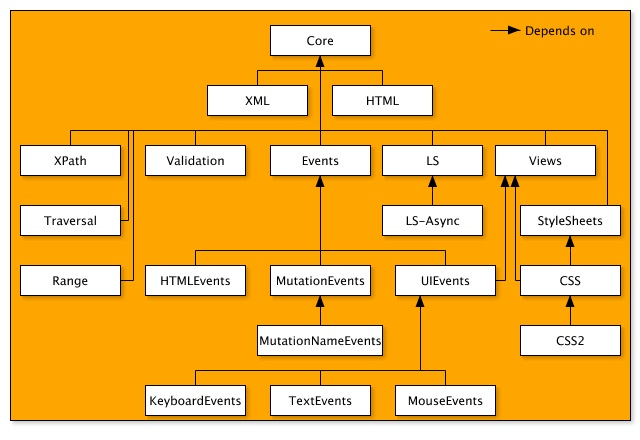
\includegraphics[width=0.45\textwidth]{figures/dom-architecture.jpg}
            \caption{Arquitectura de DOM \cite{w3c}}
            \label{fig:DOM}
        \end{figure}
        
         La interfaz de \textit{DOM} fue definida con OMG IDL y fue construida para ser usada en una gran variedad de ambientes y aplicaciones. El documento parseado por DOM se transforma en un gran objeto y el modelo no solo captura la estructura del documento si no que también el comportamiento de éste, y otros objetos de lo que puede estar compuesto y las relaciones entre ellos. Cada uno de los nodos representa un elemento parseado del documento, el cuál  posee una cierta funcionalidad e identidad. La estructura de DOM puede llegar a ser más grande que un árbol, puede llegar a almacenar más de un árbol por cada documento que parsea. %Tal estructura es possible de ser manipulado a través de scripts en las páginas, cómo JavaScript, que permite inscrustar pequeños programas usando los tag <scripr> o algún controlador de eventos de contenido.
        
\section{Javascript}
        Es un lenguaje de scripting orientado a objetos desarrollado por Netscape, siguiendo el estandar del lenguage de scripting ECMA Script. Muchos piensan que JavaScript es un lenguage interpretado, pero es más que eso. Javascript es un lenguage de scripting dinámico que soporta la construcción de objetos basados en prototipos. Esto quiere decir que a diferencia de un lenguage de programación orientado a objetos como Java, un lenguage orientado a prototipos no hace la distinción entre clases y objetos (clase instanciada), son simplemente objetos. Y cómo tal al ser construido con sus propidades iniciales, es posible poder agregar o remover propiedades, métodos de forma dinámica (durante el runtime) tanto a un objeto como a la clase.
        
        JavaScript puede funcionar tanto como un lenguage de programación procedural cómo orientado a objetos. Firefox usa una implementación en C de Javascript llamada \textit{Spider Monkey}, Google Chrome/Chromium tiene un motor de JavaScript llamado \textit{V8} e Internet Explore no usa realmente JavaScript si no que \textit{JScript} (hace lo mismo que las otras implementaciones solo que difiere en el sistema operativo que utiliza) que en este caso se llama \textit{Chakra}.
        
        Si bien es posible comprender que JavaScript posee increíbles posibilidades para la creación de \textit{RIA} (Rich Internet Applications), en \cite{barth2009attacks} se muestra que puede llegar a ser un fracaso si es que no se toman en cuenta ciertas vulnerabilidades inherentes al lenguage. Estas vulnerabilidades que pueden llegar a ser criticas, a menudo permiten a un comunicante comprometer completamente a la otra parte. La misma naturaleza de JavaScript que permite la modificación en runtime de los objetos, puede llegar a ser aprovechada de esta situación; en la cita toma por ejemplo la comunicación entre los elementos de un \textit{Mashup}.

\section{Webworkers}

\section{CORS}
Cómo lo define su nombre es un mecanismo que permite al cliente realizar request entre sitios de diverso \textit{Origen}. \textit{CORS} define una forma en que el Browser y el Servidor Web puedan interactuar para determinar si permitir o no el request a otro origen. Un Browser utiliza SOP para restringuir los request de la red y prevenir al cliente de una Aplicación Web ejecutar código que se encuentra en un origen distinto, además de limitar los request HTTP no seguros que podrían tratar de generar un daño. CORS extiende el modelo que el Browser maneja e incluye:
    
    \begin{itemize}
        \item Un header en la respuesta/response del servidor solicitado llamado \textit{Access-Control-Allow-Origin}, donde se debe escribir el origen que tendrá acceso a los recursos solicitados al servidor. Si el valor de la respuesta del servidor coincide con el \textit{origen} de quién lo solicitó, se podrá realizar el uso del recurso en el navegador, de lo contrario se generará un error.
        \item Otro header llamado \textit{Origin} pero esta vez en el request de la solicitud, para permitir al Servidor hacer cumplir las limitaciones en las peticiones de distinto origen.
    \end{itemize}
    Existen ciertos métodos en HTTP que necesitan realizar un \textit{pre-vuelo} antes de ser ejecutados, si la response del servidor es afirmativa luego se enviará el request original con el método que se debió confirmar su utilización. Para el caso de los métodos GET y POST, los más usados, este pre-vuelo no es necesario y se puede enviar el request inmediatamente.
    
    La gran diferencia de CORS con cualquier otro método de que permita hacer request hacia un origen distinto, es que el Browser por default no enviará ningún tipo de información que permita identificar al user. De esta manera se puede disminuir considerablemente las amenazas en la confidencialidad, pues el atacante no podrá hacerse pasar por un usuario del que no tiene información.
    
    Casi todos los navegadores web, a diferencia de Internet Explore \cite{bookWebAppSec}, realizan sus solicitudes a servidores de  diverso origen por medio de la interfaz \textit{XMLHTTPRequest}, en el caso de Internet Explorer esta se llama \textit{XDomainRequest}.

\section{HTTP}
\label{chap:HTTP}

\subsection{Comunicación en HTTP}
\label{chap:comunHTTP}

\subsubsection{postMessage}
\label{chap:postmessage}

\subsubsection{XMLHttpRequest}
\label{XMLHR}

\subsubsection{WebSockets}
\label{WebSockets}

